\section{Tolerance of Equipment for 1-D PDE Example}
Similar to \ref{fig:ode-convergence-std}, we demonstrate that using more sensitive measurement equipment improves the estimation of the MUD point by considering the same choices for $\tau$, the precision of the sensors.
In Figure~\ref{fig:pde-convergence-std}, we study the impact of more precise measurement equipment on the absolute error's mean and variance.


\begin{figure}[htbp]
  \centering
  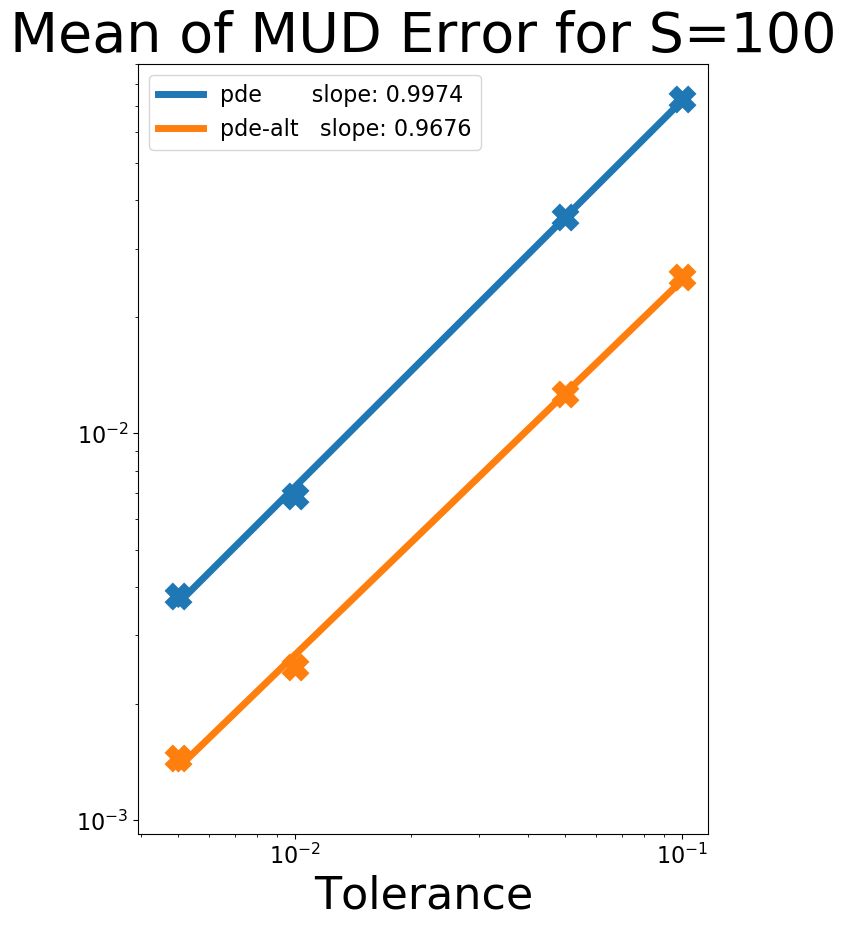
\includegraphics[width=0.475\linewidth]{figures/pde/pde_convergence_mud_std_mean}
  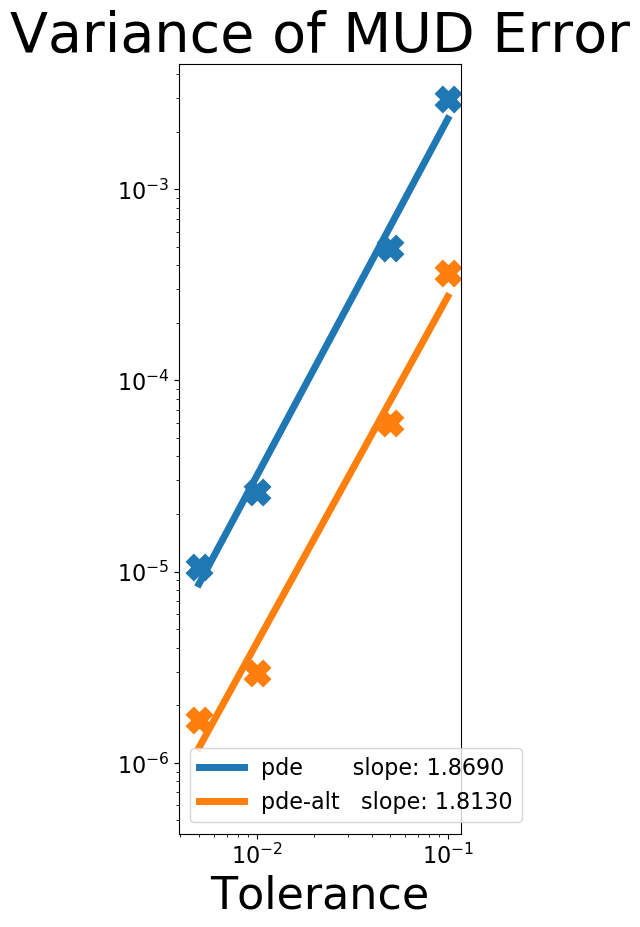
\includegraphics[width=0.475\linewidth]{figures/pde/pde_convergence_mud_std_var}
  \caption{Convergence of the MUD point given $N=1E4$ model evaluations for different measurement precision for randomly placed sensors, incorporating $S=100$ measurements.
  We note that the convergence rates are the same but the overall accuracy and precision improve when sensors are placed in regions of $u$ that exhibit higher sensitivity to changes in $\param$.
  }
  \label{fig:pde-convergence-std}
\end{figure}
